\documentclass[12pt]{article}
\usepackage[spanish]{babel}
\usepackage[utf8x]{inputenc}
\usepackage[T1]{fontenc}
\usepackage{FiraSans}
\usepackage{amsmath}
\usepackage{graphicx}
\usepackage{float}
\usepackage{subfig}
\usepackage{array}
\renewcommand{\familydefault}{\sfdefault}

\begin{document}

\begin{titlepage}
\newcommand{\HRule}{\rule{\linewidth}{0.5mm}} 
\center


\includegraphics[scale=0.4]{images/logo-usm.png}\\
\vspace{0.6cm}
\textsc{\large INF480}\\[0.5cm] % Minor heading such as course title
\textsc{\Large Redes Complejas}\\[0.5cm] % Major heading such as course name

\HRule \\[0.4cm]
{ \huge \bfseries Tarea 1}\\[0.4cm] % Title of your document
\HRule \\[1.5cm]
 
\begin{minipage}{0.8\textwidth}
\begin{center} \large
Florencia Ramírez, ROL: 202073522-0\\
Sofía Riquelme, ROL: 202073615-4
\end{center}

\end{minipage}\\[2cm]

\vfill % Fill the rest of the page with whitespace

\end{titlepage}

\section{Introducción}
En este informe se presenta un análisis de la red 6 de la lista otorgada por el profesor. Esta red proviene de una red social ``tipo Facebook'' de estudiantes de la Universidad de California en Irvine; los pesos son cantidad de mensajes entre ellos.

\section{Datos básicos}
\subsection{Cantidad de nodos y aristas}
La red cuenta con 1899 nodos y 13838 aristas.

\subsection{Dibujo}
\begin{figure}[H]
    \begin{center}
        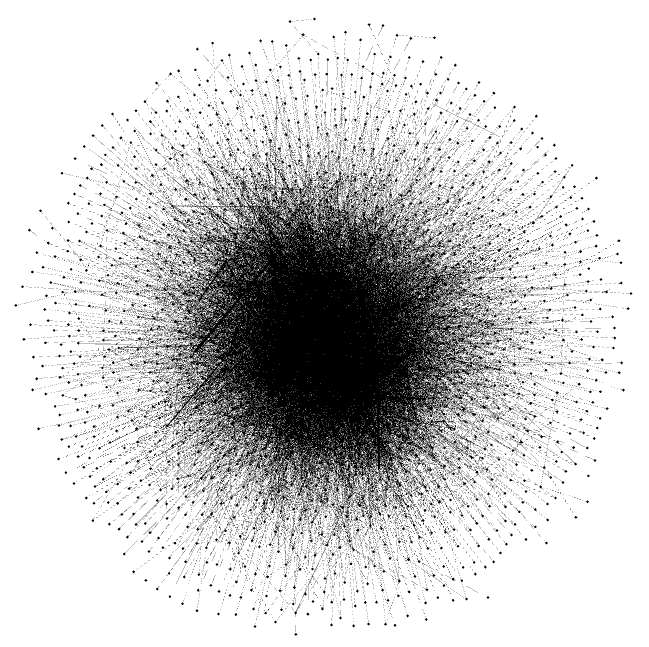
\includegraphics[scale=0.4]{images/dibujo_red.png}
    \end{center}
    \caption{Dibujo de la red}
    \label{fig:drawing}
\end{figure}

\subsection{Conexidad}
La red tiene 4 componentes conexas, donde la componente gigante representa un 99,6\% de los nodos.

\section{Análisis}

\subsection{Grados}

\begin{itemize}
    \item Grado mínimo: 1
    \item Grado máximo: 255
    \item Gráfico de distribución de grados: 
\end{itemize}
\begin{figure}[H]
    \begin{center}
        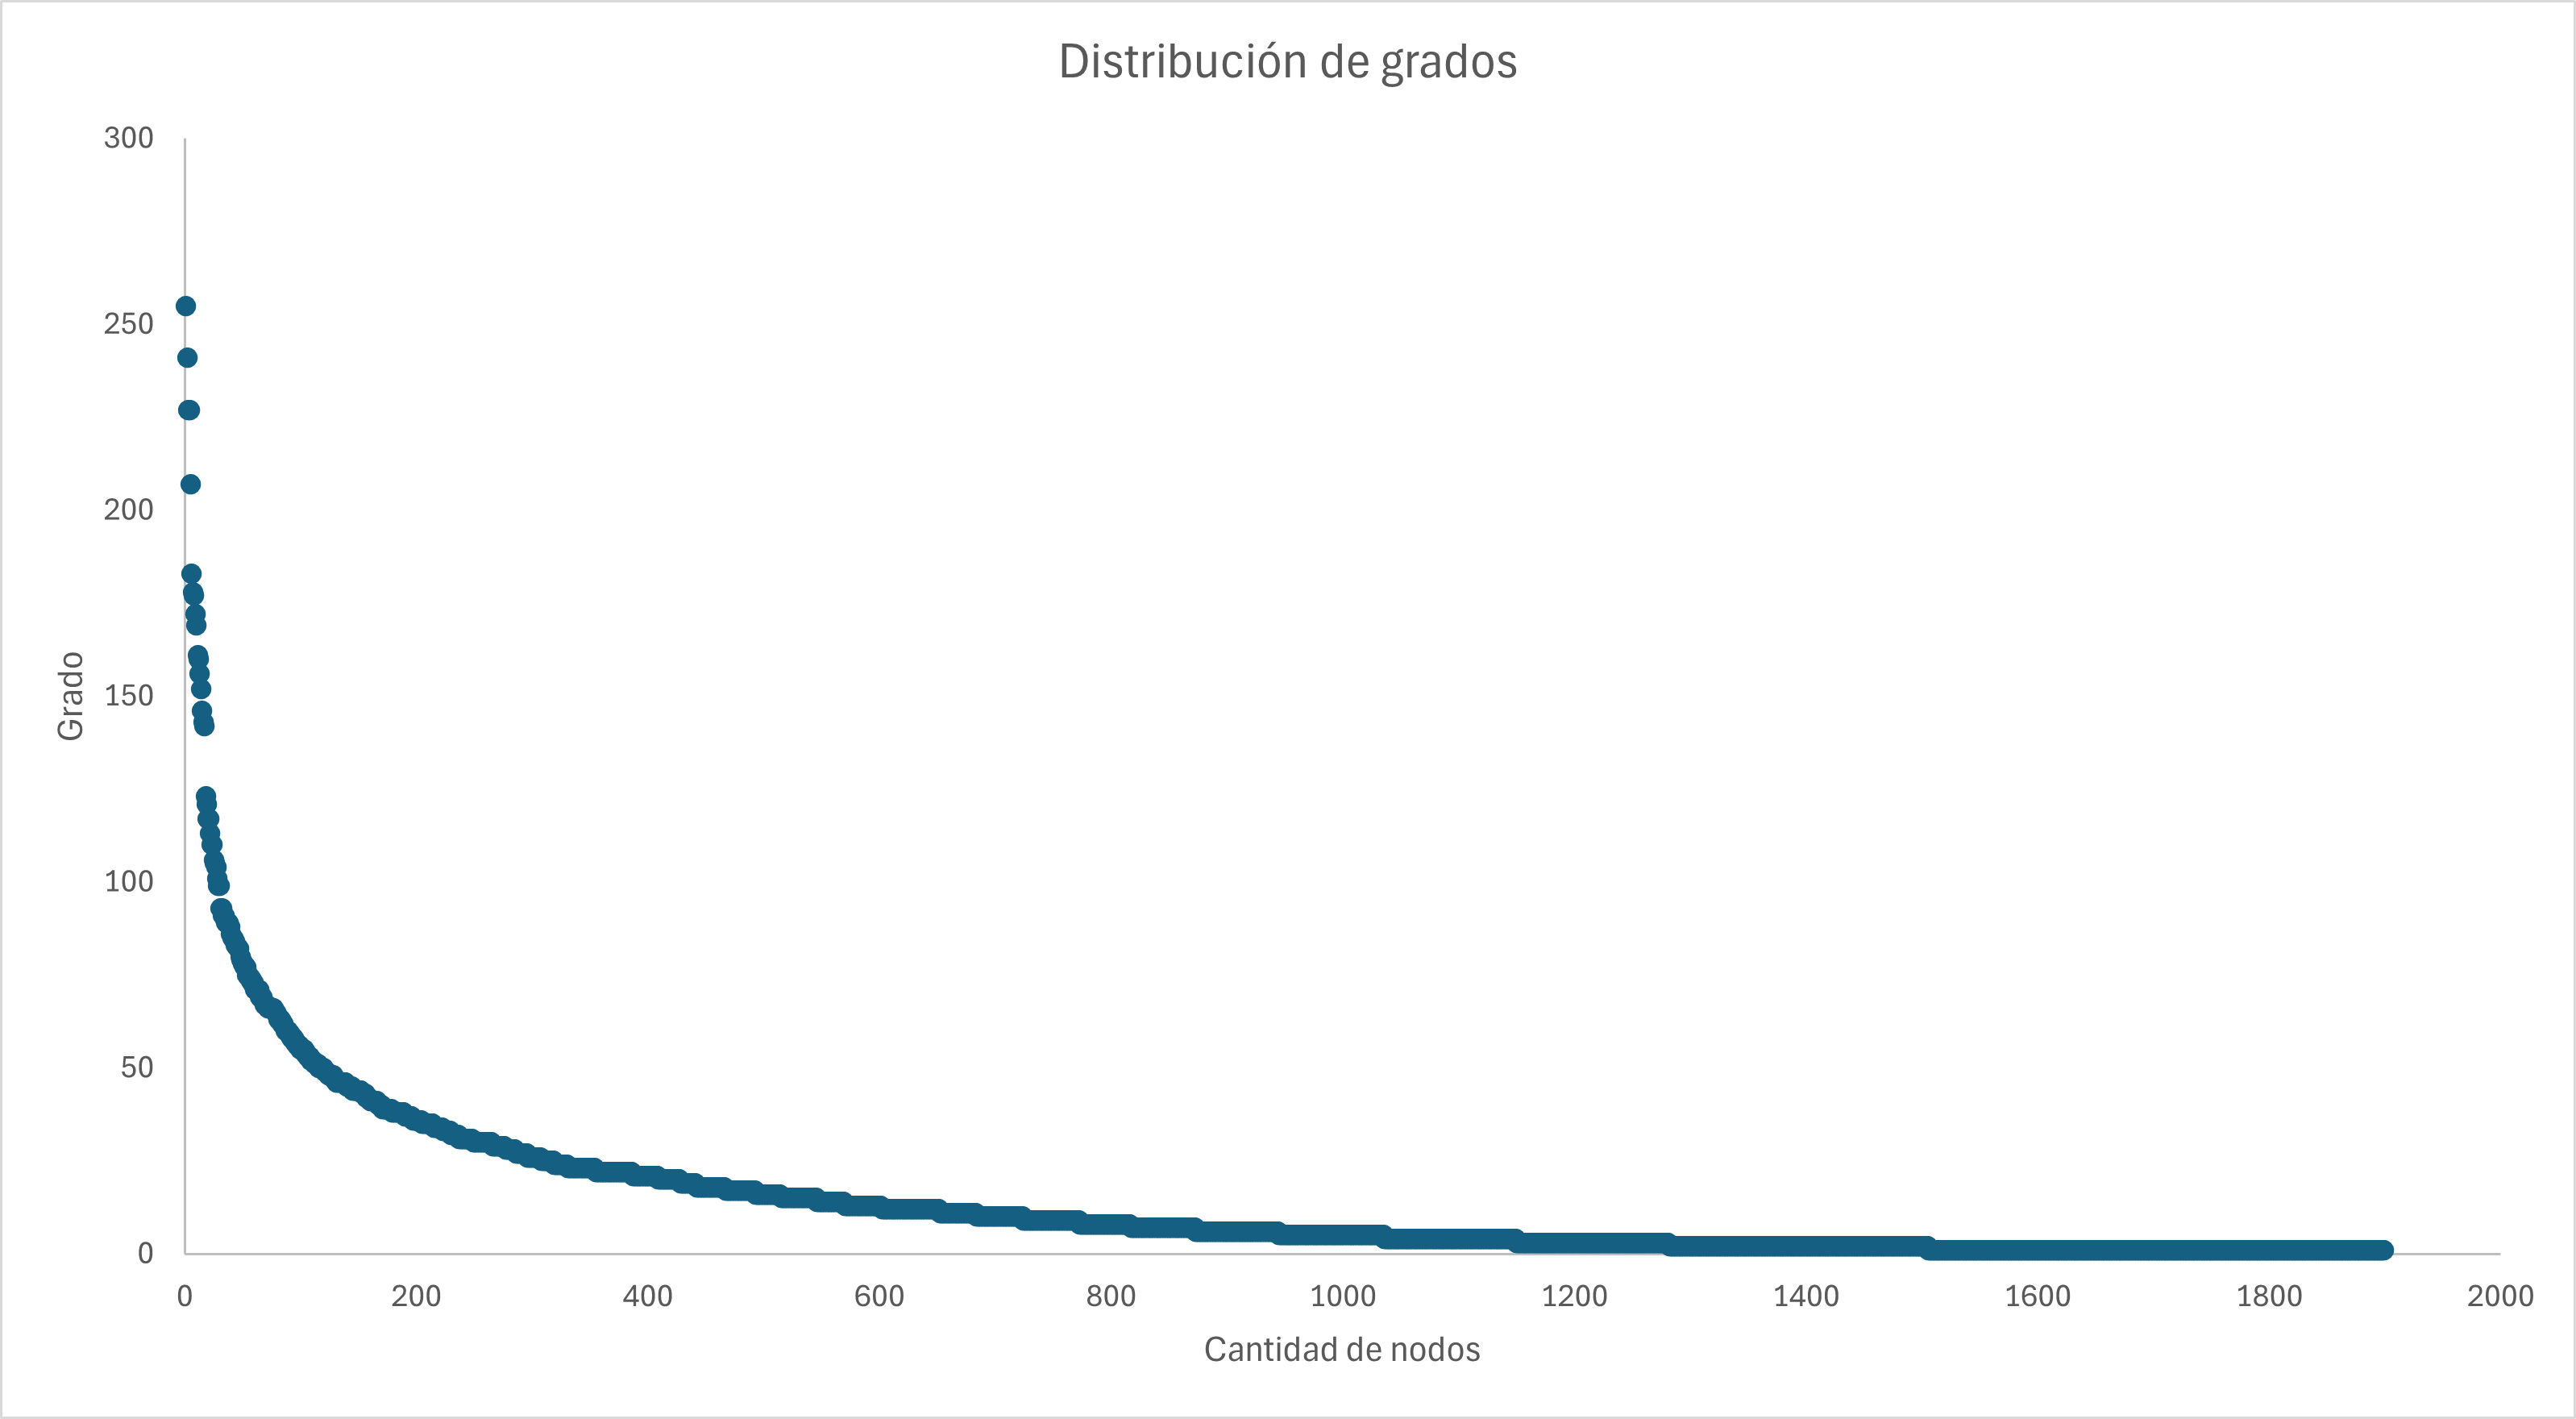
\includegraphics[scale=0.35]{images/distribucion_grados.png}
    \end{center}
    \caption{Distribución de grados}
    \label{fig:distribution}
\end{figure}
Con escala logarítmica:

\begin{figure}[H]
    \begin{center}
        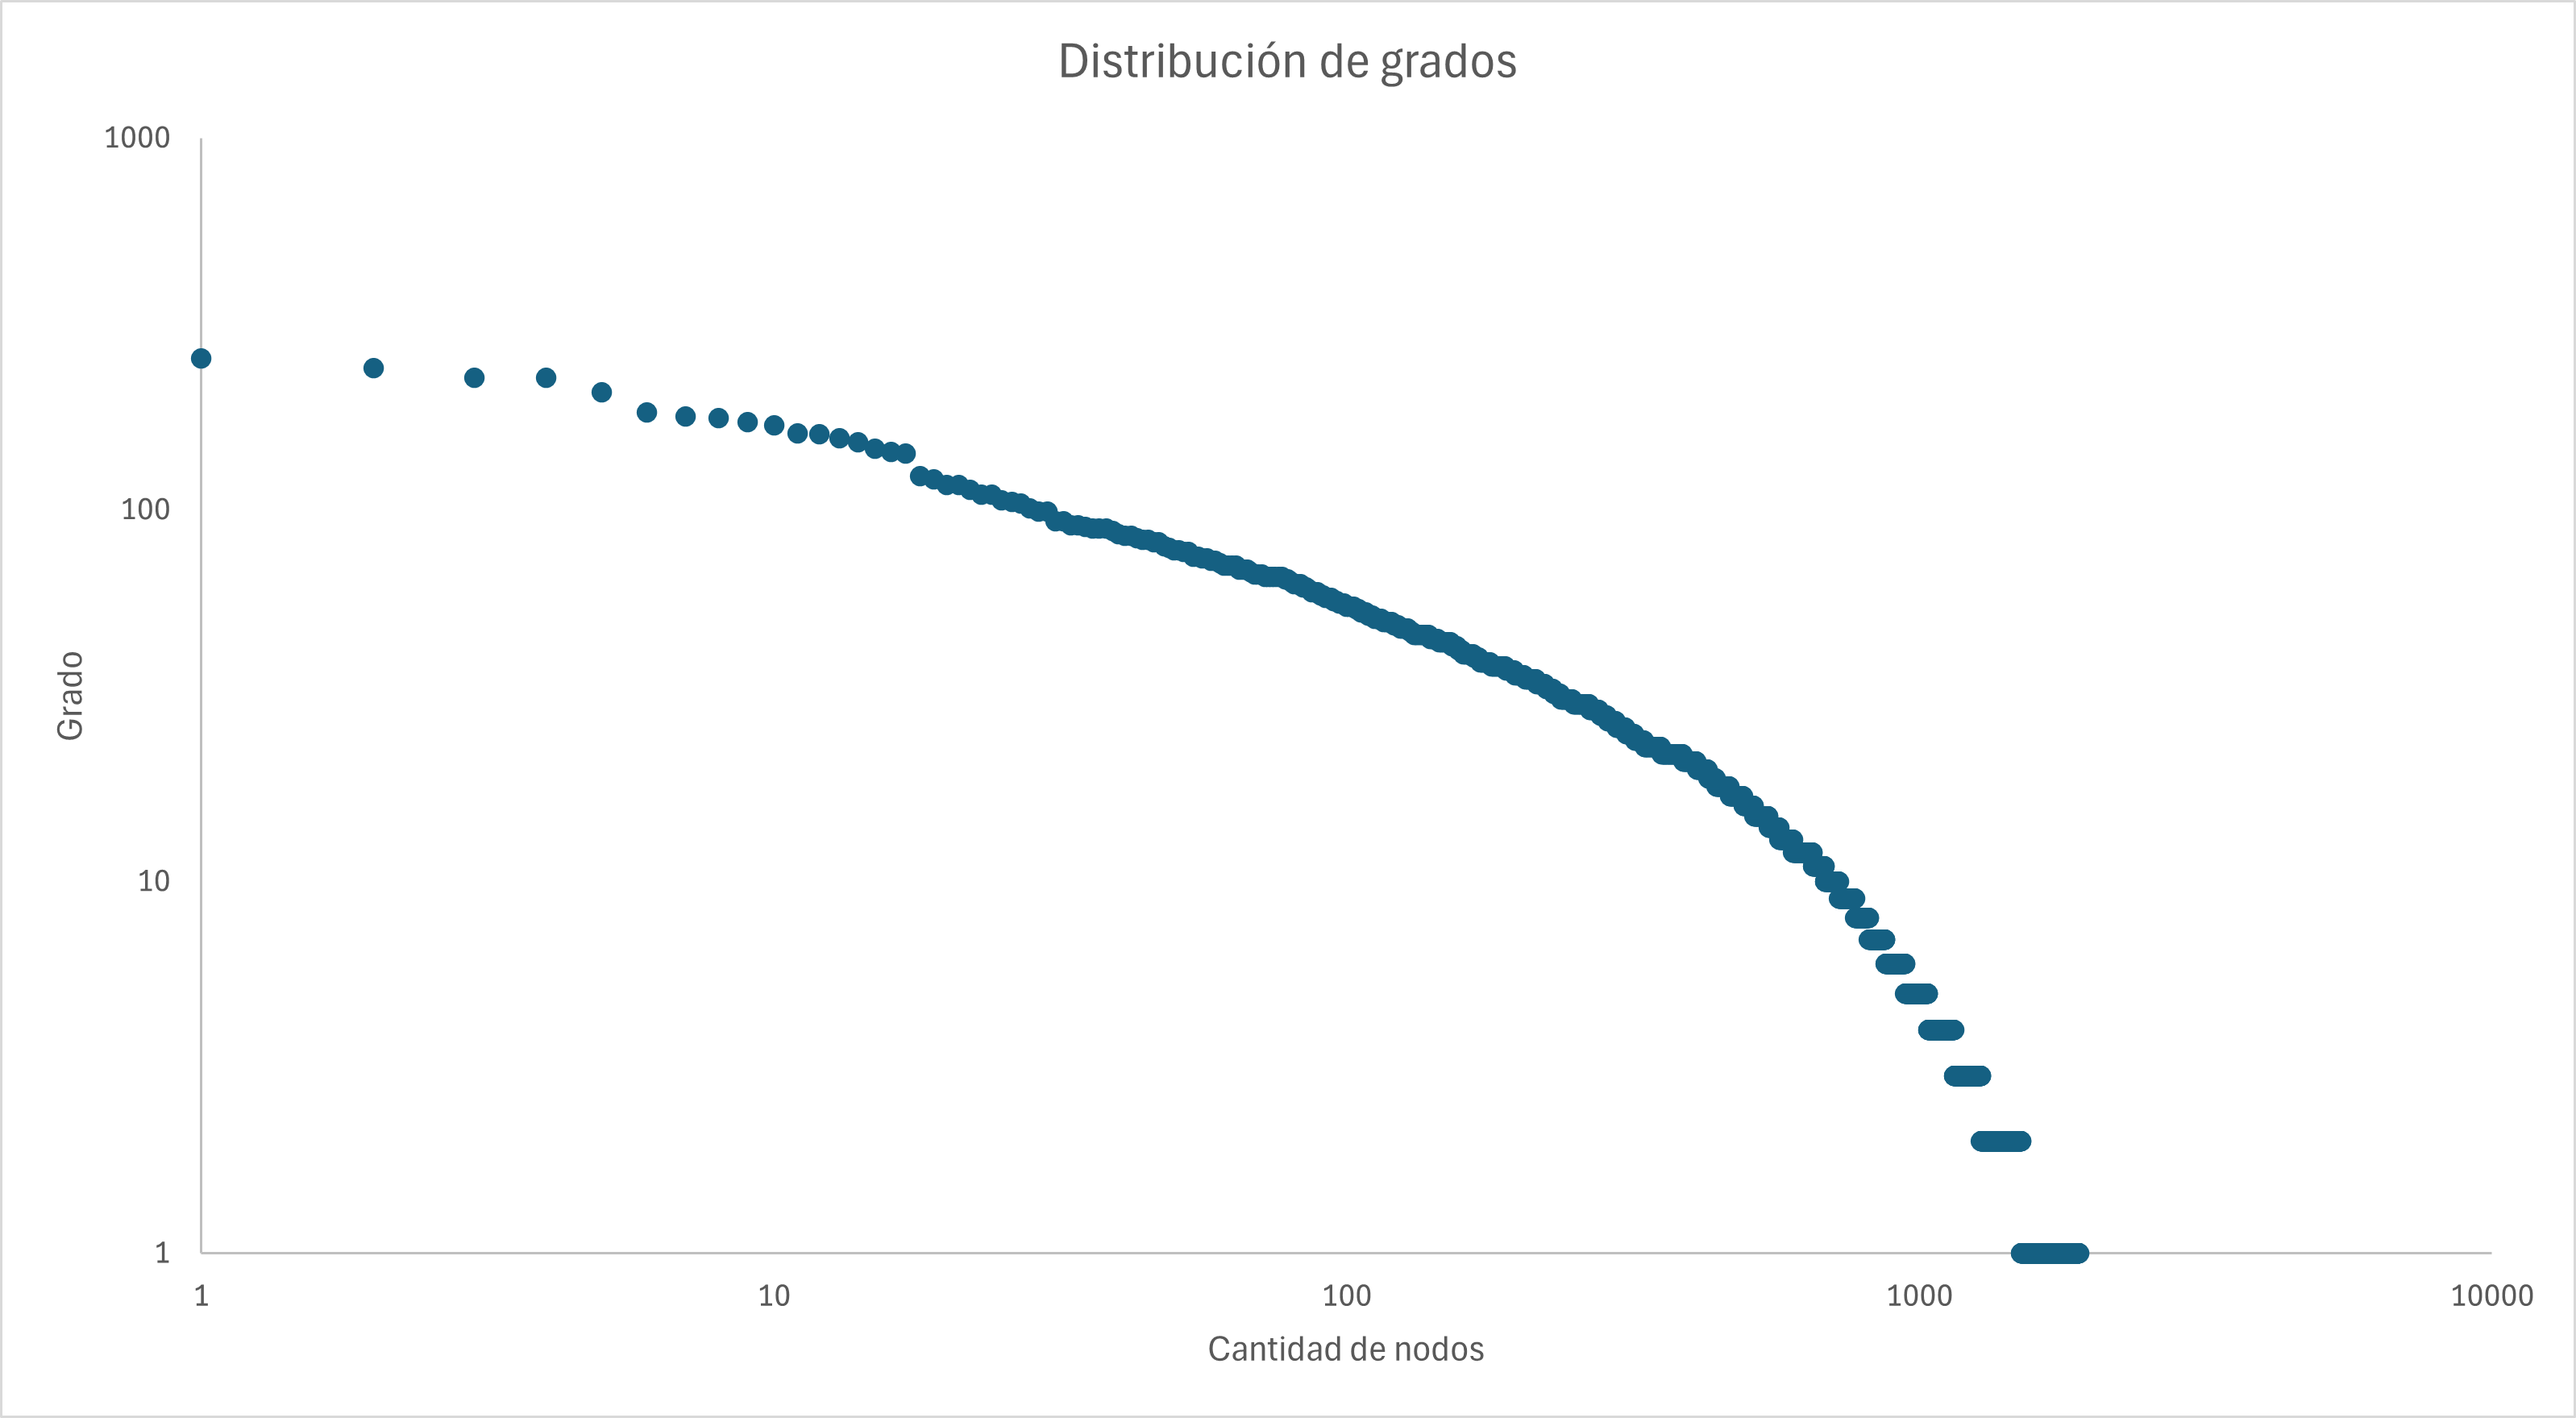
\includegraphics[scale=0.35]{images/distribucion_grados_log_log.png}
    \end{center}
    \caption{Distribución de grados en escala logarítmica}
    \label{fig:distribution-log-log}
\end{figure}

Se puede observar que si bien se esperaría que fuera una ley de potencia, no lo es.
\subsection{Distancias} 
\textit{Determine la distancia promedio entre los nodos, y el diámetro de la red. ¿Se justifica hablar de efecto small world?}

La distancia promedio entre los nodos es de 3.055 y el diámetro de la red es 8. Para justificar el efecto small world, la distancia promedio y $\log_{k} N$, que es igual a 2.813, deben ser del mismo orden de magnitud, como ambos valores son del mismo orden, se justifica hablar de small world.


\subsection{Transitividad} 
\textit{Determine el coeficiente de clustering local de la red. ¿Hay transitividad alta?}

El coeficiente de clustering promedio de la red es 0.11 y la transitividad de la red es 0.05. Esto indica que no hay un alto nivel de clustering ni tampoco una transitividad alta.


\subsection{Centralidad}  
\textit{Determine la centralidad de intermediación, PageRank y cercanía de cada nodo. Expórtelas a alguna herramienta de análisis y explore qué tan relacionadas están entre sí, y con el grado del nodo (en particular, haga gráficos de dispersión de grado y PageRank, PageRank e intermediación, etc.). Identifique las mayores desviaciones (nodos con centralidad alta según una métrica y baja según otra) e intente explicarlas en función de la estructura de la red. Obtenga imágenes de la red coloreada según los valores de las distintas centralidades. [Nota: Gephi es un poco críptico. Para calcular intermediación o cercanía hay que decirle que calcule ``diámetro de la red'', que no tiene nada que ver.]}

Luego de determinar la centralidad de intermediación, cercanía y PageRank de cada nodo, al hacer un gráfico de dispersión de grado y PageRank se obtiene lo siguiente:

\begin{figure}[H]
    \begin{center}
        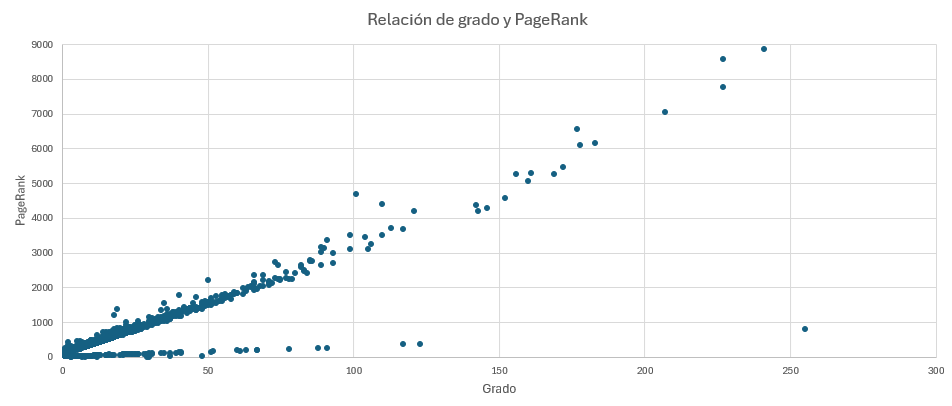
\includegraphics[scale=0.6]{images/distribucion_grado_pagerank.png}
    \end{center}
    \caption{Relación de grado y PageRank}
    \label{fig:distribution-degree}
\end{figure}

% importancia relacionada con la cantidad de conexiones
Se puede observar como en la mayoría de los casos, la cantidad de conexiones de un nodo se relaciona con la importancia que tiene este en la red. Lo que no ocurre con una cierta cantidad de estos, que a pesar de tener una cantidad considerable de conexiones, no son considerados como importantes según PageRank, ya que PageRank considera también la importancia de los nodos conectados.

Siguiendo con el gráfico de la relación entre intermediación, o betweenness, de cada nodo y su PageRank se tiene: 

\begin{figure}[H]
    \begin{center}
        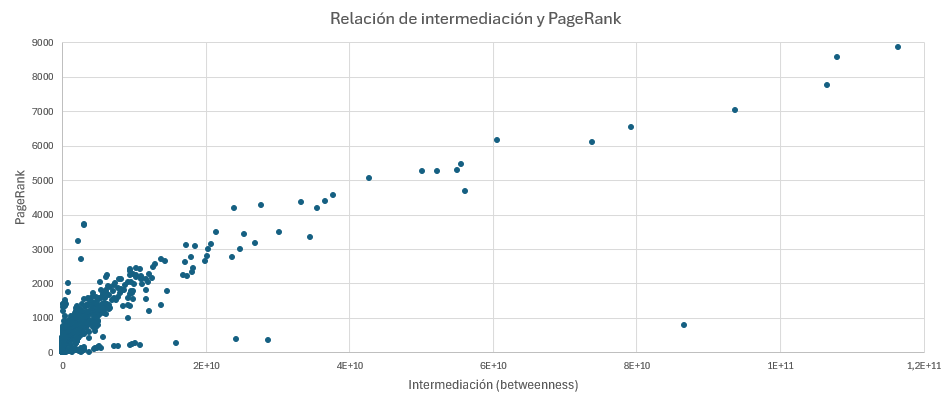
\includegraphics[scale=0.6]{images/distribucion_betweenness_pagerank.png}
    \end{center}
    \caption{Relación de intermediación y PageRank}
    \label{fig:betweenness-page-rank}
\end{figure}

% si los nodos importantes como puente son considerados importantes con el pagerank
La centralidad de intermediación de un nodo nos indica la importancia de un nodo como puente entre otros dos nodos, y se puede observar como los nodos que son considerados menos importante según PageRank, corresponden a los nodos con menores valores de intermediación, pero también existe un pequeño conjunto de nodos con un mayor valor de intermediación pero son considerados menos importantes.

Finalmente, al graficar la relación entre el grado e intermediación de un nodo se obtiene:

\begin{figure}[H]
    \begin{center}
        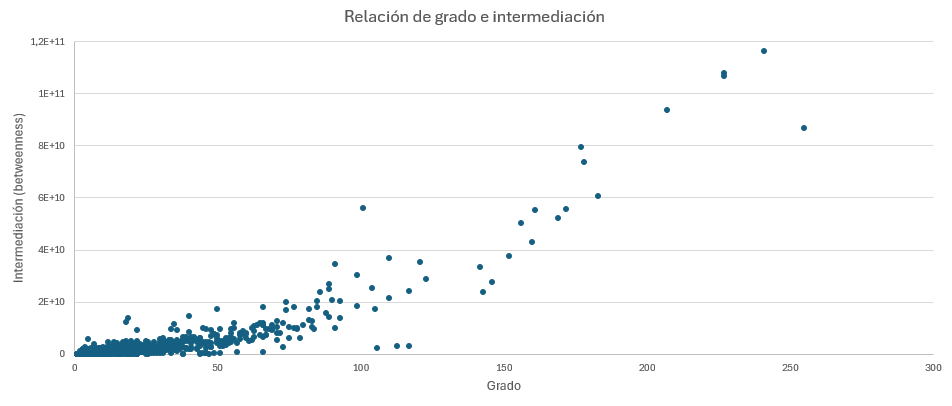
\includegraphics[scale=0.6]{images/distribucion_grado_betweenness.png}
    \end{center}
    \caption{Relación de grado e intermediación}
    \label{fig:distribution-degree-betweenness}
\end{figure}

% si nodos con grado bajo son criticos, conectando clusters o comunidades
Se puede notar como, para la mayoría de los casos, el grado del nodo está directamente relacionado con la intermediación de este. Sin embargo, se puede notar la existencia de algunas excepciones, existen nodos con menor grado que tienen un alto valor de intermediación, mientras que algunos nodos con mayor grado no tienen grandes valores de intermediación, lo que no garantiza que al tener una gran cantidad de conexiones se tenga también un gran valor de intermediación.

A continuación se muestran los distintos coloreos según los valores de cada una de las distintas centralidades:

\begin{figure}[H]
    \centering
    \subfloat[\centering Coloreo por partición]{{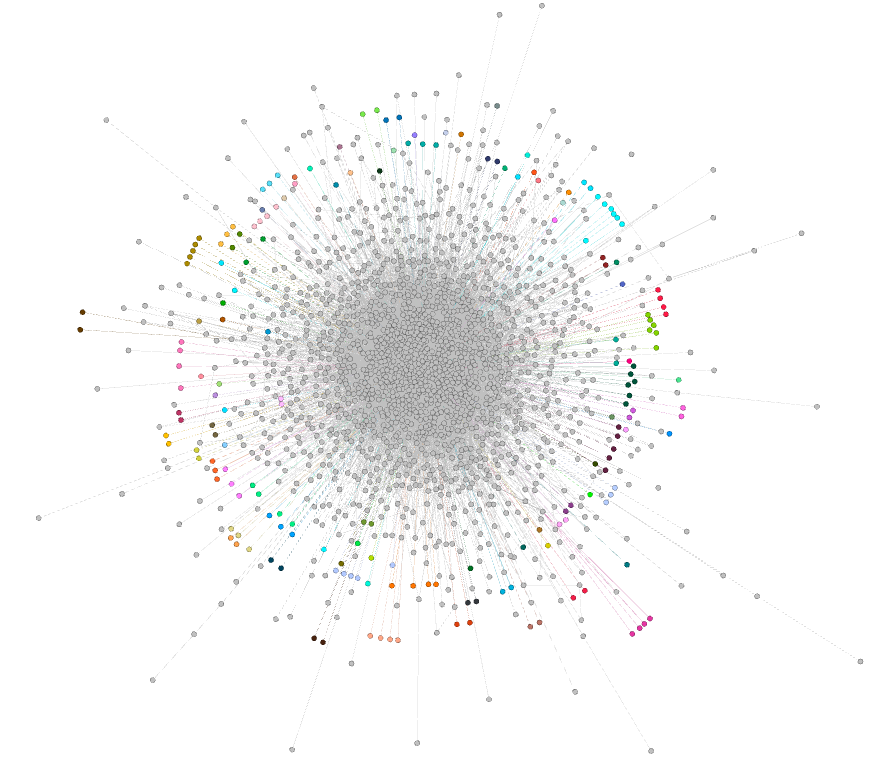
\includegraphics[scale=0.3]{images/coloreo_pagerank.png} }}%
    \qquad
    \subfloat[\centering Coloreo por ranking]{{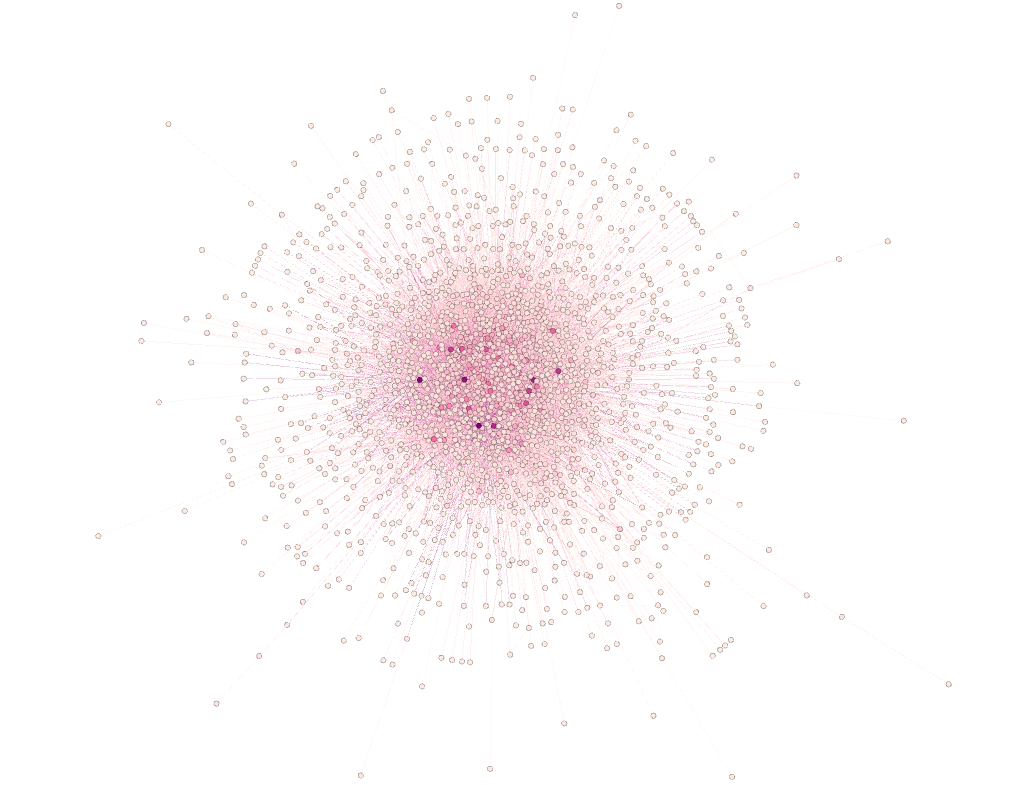
\includegraphics[scale=0.3]{images/coloreo_pagerank_v2.png} }}%
    \caption{Coloreo por PageRank}%
    \label{fig:pagerank-coloring}%
\end{figure}

\vspace{0.2cm}

\begin{figure}[H]
    \centering
    \subfloat[\centering Coloreo por partición]{{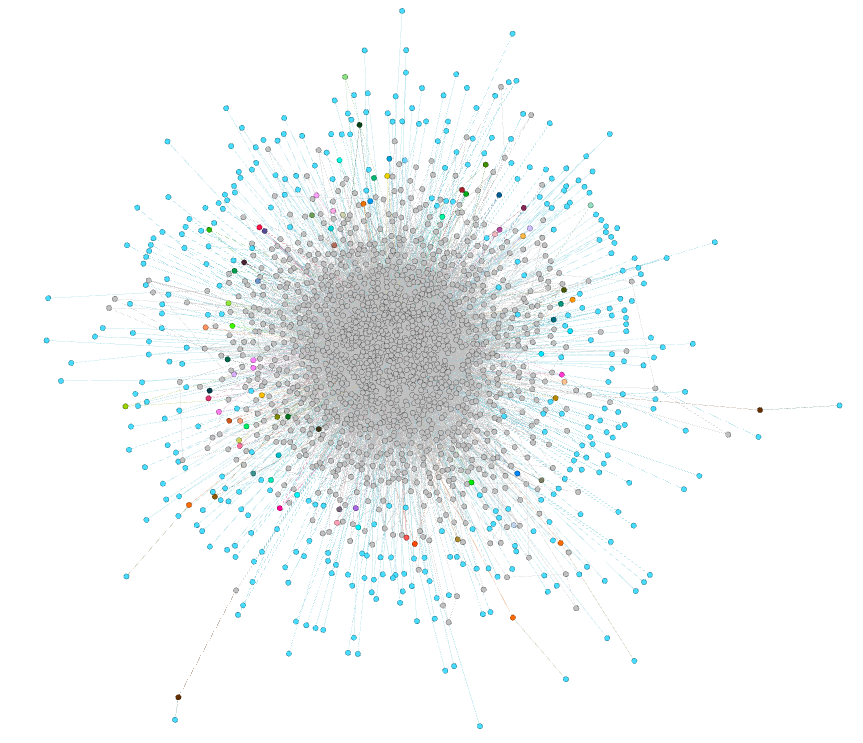
\includegraphics[scale=0.3]{images/coloreo_betweenness.png} }}%
    \qquad
    \subfloat[\centering Coloreo por ranking]{{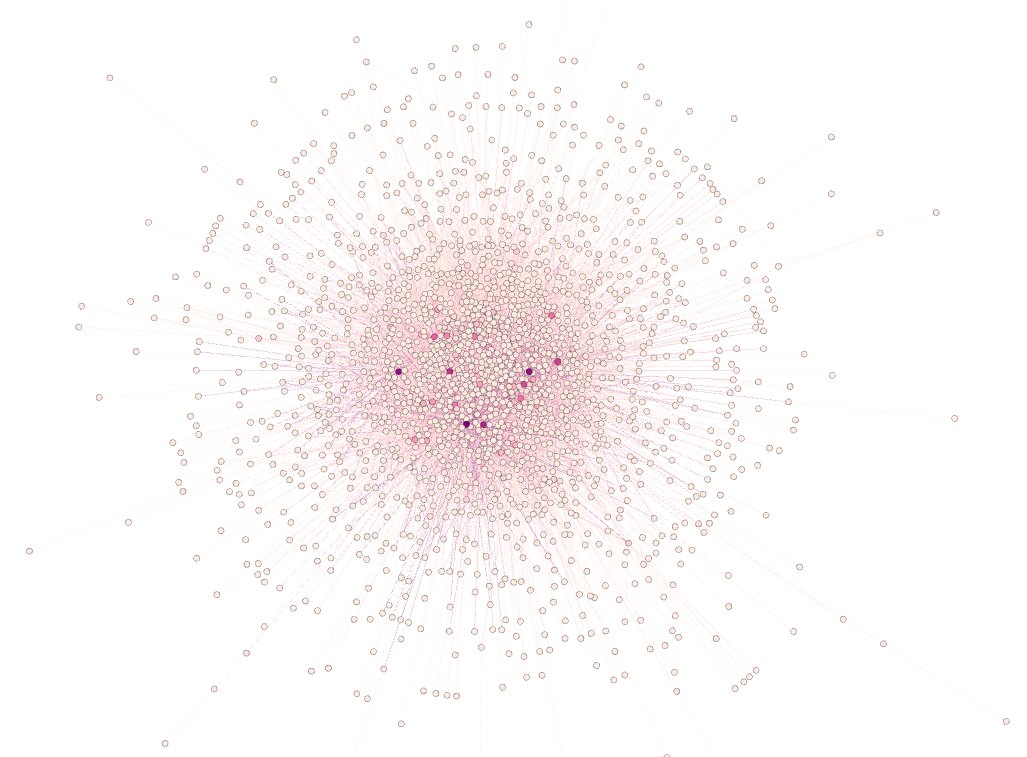
\includegraphics[scale=0.3]{images/coloreo_betweenness_v2.png} }}%
    \caption{Coloreo por intermediación}%
    \label{fig:betweenness-coloring}%
\end{figure}

\vspace{0.2cm}

\begin{figure}[H]
    \centering
    \subfloat[\centering Coloreo por partición]{{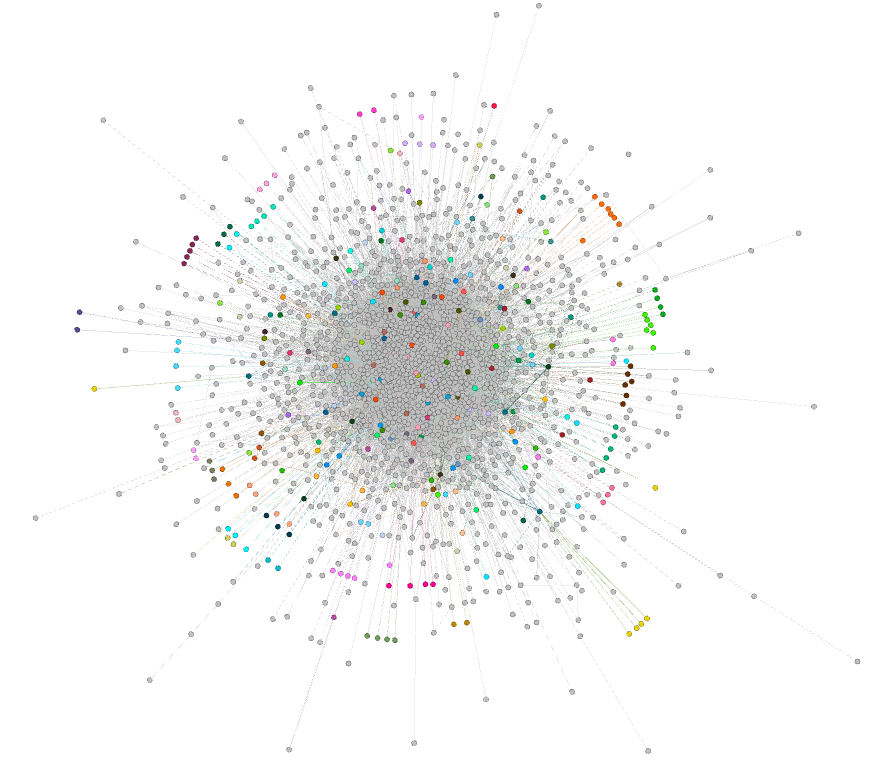
\includegraphics[scale=0.3]{images/coloreo_closeness.png} }}%
    \qquad
    \subfloat[\centering Coloreo por ranking]{{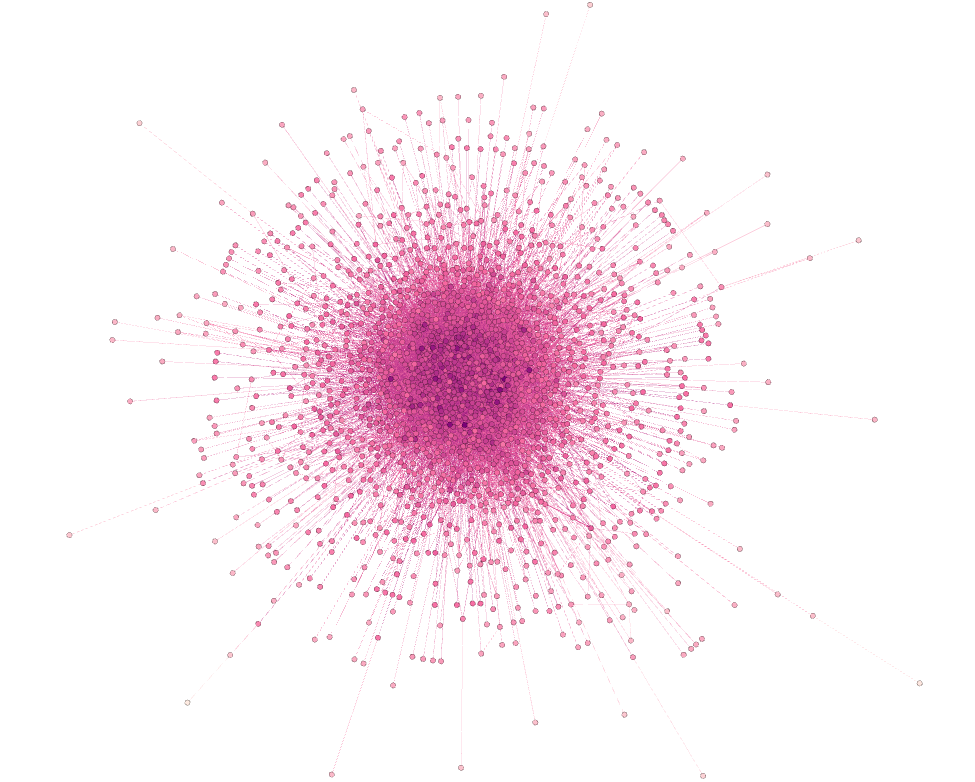
\includegraphics[scale=0.3]{images/coloreo_closeness_v2.png} }}%
    \caption{Coloreo por cercanía}%
    \label{fig:closeness-coloring}%
\end{figure}

\vspace{0.2cm}

En los coloreos de la red por partición existe una gran cantidad de particiones con un elemento, generando en total más de 1000 particiones, por lo cual existe una gran cantidad de nodos de color gris.

\newpage

\subsection{Núcleo/Periferia}
\textit{Determine la profundidad de k-cores (el máximo k para el cual el k-core es no vacío), y la cantidad de nodos en cada k-shell (cada “capa de la cebolla” en k-cores).}

La profundidad de los k-cores es 20, y para cada k-core, a continuación se adjunta una tabla con su cantidad de nodos:

\begin{table}[H]
    \centering
    \begin{tabular}{|c|c|}
        \hline
        \textbf{\( k \)} & \textbf{Cantidad de Nodos} \\ \hline
        0  & 0   \\ \hline
        1  & 395 \\ \hline
        2  & 228 \\ \hline
        3  & 141 \\ \hline
        4  & 118 \\ \hline
        5  & 100 \\ \hline
        6  & 75  \\ \hline
        7  & 54  \\ \hline
        8  & 64  \\ \hline
        9  & 59  \\ \hline
        10 & 44  \\ \hline
        11 & 57  \\ \hline
        12 & 39  \\ \hline
        13 & 32  \\ \hline
        14 & 63  \\ \hline
        15 & 54  \\ \hline
        16 & 29  \\ \hline
        17 & 53  \\ \hline
        18 & 55  \\ \hline
        19 & 32  \\ \hline
        20 & 201 \\ \hline
    \end{tabular}
    \caption{Cantidad de nodos en cada k-shell}
    \label{tab:k_shells}
\end{table}

\subsection{Comunidades} 
\textit{Aplique el algoritmo de Lovaina de detección de comunidades (Gephi lo trae por defecto). Si usa parámetros distintos al default, especifique. Reporte la cantidad y el tamaño de las comunidades encontradas, y el valor de modularidad conseguido. Use las comunidades obtenidas para colorear la red. ¿Se aprecia en el gráfico la estructura de comunidades? ¿Interactúan todas con todas, o cada comunidad se relaciona con unas pocas de las demás? [Aquí si hace falta puede jugar un poco más con las opciones de layout, para buscar un buen dibujo de la red.]}

Se obtuvieron 15 comunidades distintas, con una modularidad de 0.355. A continuación se presenta una imagen coloreada por comunidad:

\begin{figure}[H]
    \begin{center}
        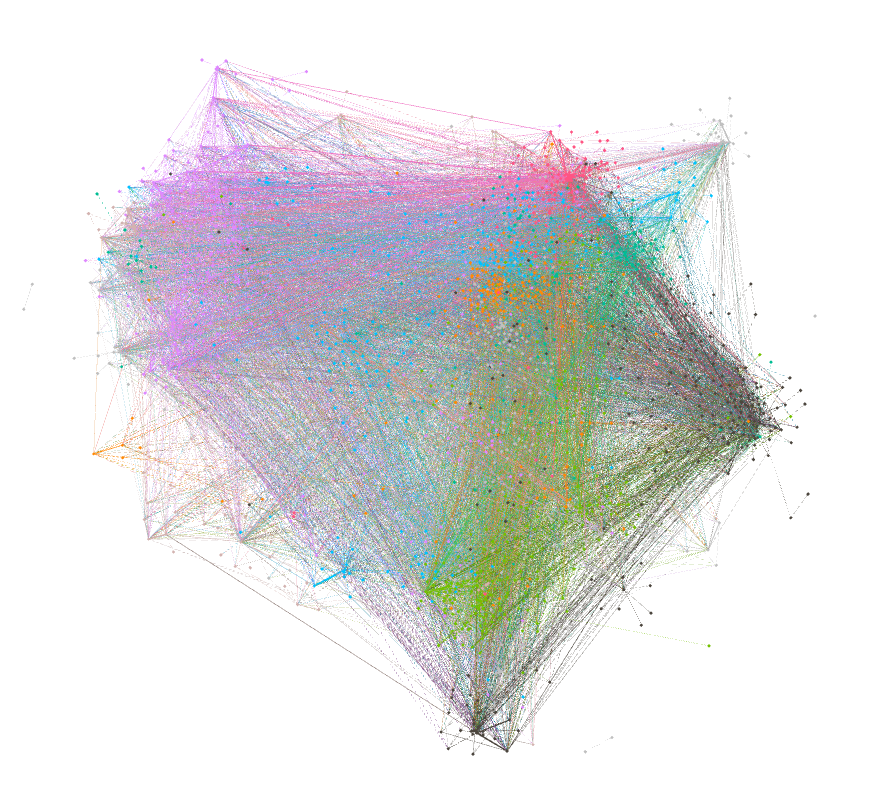
\includegraphics[scale=0.4]{images/red_comunidades.png}
    \end{center}
    \caption{Imagen coloreada por comunidad}
    \label{fig:drawing-community}
\end{figure}
\subsection{Asortatividad}
\textit{Calcule el coeficiente de correlación de Newman para medir la asortatividad de la red. ¿Le parece asortativa, disasortativa, o ninguna?}

El coeficiente de correlación de Newman es -0.18 para esta red. Esto indica que es disasortativa (por ser un valor negativo), sin embargo, no está lo suficientemente cerca de -1 como para ser completamente disasortativa.

\subsection{Modelo estructural} 
\textit{Genere 10 redes aleatorizadas que compartan la distribución de grados de su red, y para cada una de ellas determine la modularidad (aplicando el mismo algoritmo de Lovaina), el coeficiente de correlación, el coeficiente de clustering local, y la profundidad de k-cores. Compare los valores con el obtenido para su red: ¿pueden explicarse sus valores a partir de la distribución de grados, o parecen ser propiedades específicas de la red?}
A continuación se presenta una tabla con los valores obtenidos al generar 10 redes aleatorias:
\begin{table}[H]
    \centering
    \begin{tabular}{|c|c|c|c|c|}
        \hline
        No. & Modularidad & Correlación & Clustering & k-cores \\
        \hline
        1  & 0.2058 & -0.0477 & 0.0665 & 18 \\
        2  & 0.2099 & -0.0412 & 0.0670 & 18 \\
        3  & 0.2054 & -0.0479 & 0.0706 & 18 \\
        4  & 0.2094 & -0.0467 & 0.0723 & 19 \\
        5  & 0.2081 & -0.0528 & 0.0686 & 18 \\
        6  & 0.2036 & -0.0444 & 0.0667 & 18 \\
        7  & 0.2040 & -0.0533 & 0.0694 & 18 \\
        8  & 0.2076 & -0.0547 & 0.0685 & 18 \\
        9  & 0.2066 & -0.0288 & 0.0634 & 19 \\
        10 & 0.2105 & -0.0430 & 0.0690 & 18 \\
        \hline
    \end{tabular}
    \caption{Análisis de redes aleatorizadas}
    \label{tab:redes_aleatorizadas}
\end{table}
Considerando los valores de la tabla anterior, se puede observar lo siguiente:
\begin{itemize}
	\item Modularidad: En la red original la modularidad es de 0.355 mientras que en las redes aleatorizadas varían entre 0.2036 y 0.2105. Dado que esta es una variación significativa de la red original, indica que hay características específicas de la red que generan estos valores.

	\item Profundidad de k-cores: En la red original son 20 y en las aleatorizadas varía entre 18 y 19. Estos valores son bastante cercanos entre sí, por lo que sí se podría explicar por la distribución de grados.

	\item Coeficiente de clustering: En la red original el coeficiente es 0.11, y en las redes aleatorias varían entre 0.0634 y 0.0723. Esto sugiere que el coeficiente de clustering de la red original no puede explicarse simplemente por la distribución de grados.

	\item Correlación de grado: En la red original se tiene un coeficiente de correlación de  -0.18 mientras que en las redes aleatorias varían entre -0.0288 y -0.0547. La red original tiene una correlación de grado más negativa que las redes aleatorizadas, indicando que la tendencia de nodos de alto grado a conectarse con nodos de bajo grado es más pronunciada en la red original que en las aleatorizadas.
\end{itemize}
\end{document}